%%%%%%%%%%%%%%%%%%%%%%%%%%%%%%%%%%%%%%%%%%%%%%%%
% COPYRIGHT: (C) 2012-2015 FAU FabLab and others
% CC-BY-SA 3.0
%%%%%%%%%%%%%%%%%%%%%%%%%%%%%%%%%%%%%%%%%%%%%%%%


\newcommand{\basedir}{fablab-document}
\documentclass{\basedir/fablab-document}

% \usepackage{fancybox} %ovale Boxen für Knöpfe - nicht mehr benötigt
\usepackage{amssymb} % Symbole für Knöpfe
\usepackage{subfigure,caption}

\usepackage{eurosym}
\usepackage{tabularx} % Tabellen mit bestimmtem Breitenverhältnis der Spalten
\usepackage{wrapfig} % Textumlauf um Bilder
\renewcommand{\texteuro}{\euro}

\linespread{1.2}

\date{2014}
\author{Max, Philipp, Michael u.a.}
\fancyfoot[L]{kontakt@fablab.fau.de}
\title{Grundlagen-Einweisung Fräse}

\tikzstyle{knopf} = [anchor=base, draw=black, fill=gray!10, rectangle, rounded corners, inner sep=2pt, outer sep = 3pt]

\newcommand{\knopfStyled}[2]{
    \begin{tikzpicture}[baseline={(box.base)}]
    \node [#1] (box) { 
        \fontsize{9pt}{9pt}\selectfont \textbf{#2}\strut
    };
    \end{tikzpicture}
}

\newcommand{\knopf}[1]{\knopfStyled{knopf}{#1}}
\newcommand{\cncStart}{\knopf{Start}}

%\tikzstyle{todo} = [knopf, draw=white, fill=yellow]
%\newcommand{\todo}[1]{\knopfStyled{todo}{#1}}
\renewcommand{\todo}[1]{\colorbox{yellow}{{#1}}}

\usetikzlibrary{shadows}
\usetikzlibrary{decorations}
\begin{document}
\section{Regeln und Hinweise}\label{regeln}
\subsection{Was darf ich?}
Ohne eine unterschriebene Grund-Einweisung in diese Regeln darf die Fräse nicht benutzt werden, d.h. du darfst \emph{garnichts} an/in der Fräse und dem zugehörigen Steuerrechner tun.
\begin{itemize}
 \item Jede Einweisung verfällt nach einem Jahr, wenn sie nicht vorher schriftlich erneuert wurde. 
 \item Mit Grund-Einweisung darfst du den Fräs-Auftrag zwar selber vorbereiten (Werkstück einspannen), \textbf{die Steuerung aber nicht selbstständig bedienen, also die Maschine nicht \enquote{fahren lassen}}.
 \item Alles andere darfst du zuerst nur unter ständiger Aufsicht durch einen Experten. Mit jedem Fräsen lernst du dazu und darfst dann immer mehr selbstständig tun, sobald es dir \textbf{schriftlich} erlaubt wird:
 %\item Die Bedienung der Steuersoftware (Antasten, Starten, Fortsetzen nach Pause, ...) darf nur durch den Experten bzw. unter ständiger Aufsicht durch den Experten erfolgen.
\end{itemize}
\colorlet{blockhintergrund}{blue!50!gray}
\tikzstyle{lernstufe} = [rectangle, draw, thick, top color=blockhintergrund!10,bottom color=blockhintergrund!30, draw=blockhintergrund!70!black,
    text width=16em, text centered, rounded corners, minimum height=4em, drop shadow]
\tikzstyle{pfeilLernen} = [draw,->, thick, every node/.style={text width=38em}]
%\begin{figure}
\vspace{1em}
\begin{tikzpicture}[scale=0.8, node distance = 3cm, auto]
\newcommand{\ueb}[1]{\textbf{#1}\\}
 \node[lernstufe] (0) {\ueb{Stufe 0: garnichts} Fräse nicht anfassen, nur bestaunen :)};
 \node[lernstufe, below of = 0, node distance=3cm] (1) {\ueb{Stufe 1: Anfassen} Ein-/Ausspannen, Säubern.\\Nichts alleine an der Steuerung.};
 \node[lernstufe, below of = 1, node distance=4.7cm] (2) {\ueb{Stufe 2: Handbetrieb}  Manuelles Verfahren, Einrichten.\\Nicht starten oder wiederfortsetzen.};
\node[lernstufe, below of = 2, node distance=7.2cm] (3) {\ueb{Fräsenbetreuer: Alles} auch Starten, Freigabe,\\ Einweisung anderer Nutzer};
\path[pfeilLernen] (0) -- node {Arbeitssicherheit und Ordnung (Kapitel \ref{regeln} Regeln und Hinweise)\\Grund-Einweisung mit Unterschrift} (1);
\path[pfeilLernen] (1) -- node {Benutzung der Spannmittel üben: Pratzen, Schraubstock, Vakuumtisch \todo{sobald in Betrieb}\\
Einrichten unter Aufsicht erlernen:  Handbedienung, Nullpunkt, Spannzange, Werkzeugwechsel,
Absaugvorrichtung \todo{(sobald es sie gibt)}, Längenmessung, Spindel vorheizen, Kühlmittel,  Prüfen vor dem Start, ...\\[0.5em]
	Einweisung mit Unterschrift, sobald Einrichten sicher beherrscht} (2);
\path[pfeilLernen] (2) -- node {Bezahlung, NC-Programm erstellen, Auswahl der Fräser, Verständnis der Zerspanung (u.a. Gleichlauf/Gegenlauf, Belastung beim Nutfräsen, Schnittdaten, Fräserliste, Datenblatt)\\[0.5em]
	Üben und Routine bekommen, Aufsicht ist weiterhin zum Start notwendig.\\[0.5em]
	Einweisung vollständig verstanden haben und so sicher selbstständig arbeiten können,
	dass die Aufsicht nicht mehr helfen oder eingreifen muss.\\[0.5em]
	An verschiedenen Tagen mehrere verschiedenartige Werkstücke erfolgreich fräsen\\[0.5em]
	Schriftliche Bestätigung durch Betreuer und Teilnehmer: \enquote{Führerschein}\\Herzlichen Glückwunsch, du bist jetzt auch Fräsenbetreuer!} (3);
\end{tikzpicture}
% \vspace{-20em}
% 
%\pagebreak
%\end{figure}


\subsection{Handhabung}
\begin{itemize}
 \item Die Fräse ist ein kompliziertes und teures Gerät; eine Anleitung dazu kann nie vollständig sein. Nachdenken, Sorgfalt und Vorsicht sind nötig, damit weder Menschen noch die Maschine zu Schaden kommen.
 \item Mache dich mit den Schutzeinrichtungen (Türschalter, Notaus, ESC / Pause am PC, Begrenzungen in der Steuerung) und ihren Einschränkungen vertraut. Dabei sollte dir auch klar werden, wieso und wann
\begin{itemize}
 \item es nach dem Not-Aus oder Türe öffnen noch etwas dauert, bis ein sicherer Zustand erreicht ist,
       % -> Nachlauf der Spindel. Bei Handbetrieb kann man auch den Zustand Spindel an + Tür auf erreichen!
 \item die ESC- und erst recht die F4-Taste am PC kein Ersatz für den Not-Aus ist
       % -> Wenn der PC abstürzt, geht garnichts davon. F4 nur im laufenden Programm, nicht beispielsweise wenn die Werkzeuglängenmessung Amok läuft
 \item die Steuerung nicht immer verhindern kann, dass der Fräser in den Nutentisch rammt
       % -> Sie kennt die Werkzeuglänge nicht
\end{itemize}

 \item Die beschriebenen Abläufe müssen unbedingt beachtet werden. Bei Unklarheiten nachfragen!
 \item Beim Hantieren in der Fräse:
	\begin{itemize}
	\item Schmiermittel und Späne sind nicht gut für die Haut. Einweghandschuhe sind in der Werkbank.
	\item Beim Ausblasen für Augenschutz (Späne) und ggf.\  Gehörschutz sorgen. Ausblasen verteilt oft nur den Dreck, deshalb lieber kehren oder saugen. Es besteht die Gefahr, dass Dreck in abgedichtete Bereiche, z.\,B.\  unten bei der Spindel, gepresst wird.
	\item Während jemand an der offenen Fräse ist, bedient kein anderer den PC. Zum manuellen Verfahren beim Antasten die Tastatur mitnehmen und es selber machen!
	\item Spindel und Nebelkühlung auslassen, solange die Maschine offen ist!
	\item Ausnahme Kühlung: beim Justieren der Kühlmittelstrahlen auf den Fräser darf die Kühlung natürlich an sein.
	\end{itemize}
 \item Materialien, die leitfähigen oder abrasiven Staub erzeugen, sind vorerst nicht erlaubt (unter anderem Graphit, Carbon, Stein, GFK, Platinen)
 \item Die Deckenlüftung muss an sein, solange die Fräse in Benutzung ist.
 \item Bei Bruch eines Fräsers muss der in der Tabelle stehende Kostenanteil gezahlt werden, unabhängig von einem Verschulden des Benutzers. (Irgendwo muss das Geld für den neuen Fräser ja herkommen.)
\end{itemize}
\subsection{Ordnung} \label{ordnung}
\begin{itemize}
\item Bei den Spänen auf Mülltrennung achten: Normalerweise sind Aluspäne in der Wanne. Wenn Eisen gefräst wird, Wanne davor und danach in den passenden Eimer ausleeren.
\item Nach Öffnen der Türen ist zu kontrollieren, ob Späne auf den Boden neben der Rutschmatte gefallen sind. Wenn ja, \emph{sofort} wegsaugen.
 \item Auch die Türkanten absaugen (verhindert von Anfang an, dass Späne auf den Boden fallen)
 \item Nach getaner Arbeit Fräse wieder schön sauber machen:
	  \begin{itemize}
	    \item Werkstück ausspannen und abwaschen
	    \item Türkanten saugen
	    \item Spannmittel abwaschen, abtrocknen und aufräumen
			\item Nutentisch abkehren (Augenschutz!)
	    \item Nutentisch nach hinten abblasen (Augenschutz! Gehörschutz!)
	    \item Späne in die Spänewanne kehren oder wegsaugen
	    \item Kühlmittel-Ausströmer saubermachen, damit man sich beim Einstellen nicht die Hände zersticht oder vollsifft
	    \item Scheibe der Haupttür soweit saubermachen, dass man den Fräser gut beobachten kann. Dies muss mit nassen Tüchern besonders vorsichtig gemacht werden, um die Scheibe nicht mit Spänen zu zerkratzen
			\item Spänewanne in den richtigen Eimer ausleeren
			\item Boden rund um die Fräse saugen, wenn Späne rausgefallen sind
	  \end{itemize}
 \item Vor dem Ausschalten: Tisch in Parkposition fahren (\knopf{P2} im Referenzfahrt-Menü)
\end{itemize}


\section{Checkliste Auftragsstart}
\subsection{CAM}
\begin{enumerate}
 \item Herausfallende Stücke? Stege setzen.\\Richtwert: bei Alublech alle 50-100mm ein 2mm dicker und 2mm langer rechteckiger (nicht angeschrägter) Steg. Je nach Fräserdicke und Material muss das angepasst werden.\\
VCarve: Wenn tiefer gefräst wird als das Material, muss die Stegdicke entsprechend erhöht werden, denn diese bezieht sich immer auf den untersten Punkt der Fräsung. Vorsicht auch bei unebenem Material.
 \item VCarve: Starttiefe=0, wenn nicht vorher mindestens so tief ausgefräst (Reihenfolge!)\\
Für besondere Vorsicht (unebenes Material) kann Starttiefe auch negativ sein.
 \item VCarve: Frästiefe $<$ nutzbare Schneidenlänge (bzw. Freistellungslänge) des Fräsers? (siehe Fräsertabelle oder Datenblatt)\\ (Bei Schaum u.\,ä.\  kann ein gleich dicker Schaft auch ausreichend sein) \\
 Wird tiefer als die Schneidenlänge gefräst, ist beim Nutfräsen besonders auf die Spanabfuhr zu achten. \\
 Sollten sich Späne in der Nut sammeln, Job pausieren und mit Druckluft ausblasen.
 \item Ist der Fräser stirnseitig schneidend? (Fräsertabelle oder Datenblatt) Wenn nein, darf er nicht bohren oder senkrecht eintauchen.\\
(Beispiele zur Zeit: Och Fräser in Edelstahl und Titan, ..., Sonderfall Entgratfräser: nur die Spitze kann nicht bohren)\\
Diese Fräser sind oft, aber nicht immer, im VCarve extra gekennzeichnet.\\
Dann möglichst einen anderen Fräser verwenden oder im VCarve: Schrägeintauchen/Anfahrrampe aktivieren, außerdem die Stege rampenförmig und nicht rechteckig einstellen (Eintauchrampe gilt nicht für Stege!)  \todo{prüfen ob das wirklich ausreicht}\\
Den erzeugten Werkzeugweg kritisch anschauen, ob er wirklich immer schräg verfährt.
 \item unabhängig davon ist ein schräges Eintauchen fräserschonender (VCarve: Anfahrrampe schräg, Länge der Anfahrrampe ungefähr gleich der Eintauchtiefe wählen.)
 \item VCarve Bohren: wenn Fräser zum Bohren verwendet werden oder relativ tief gebohrt wird, Tieflochbohren mit 1mm Rückzugshöhe aktivieren (Bohrer wird nach der eingestellten Bearbeitungstiefe ganz (+1mm) herausgefahren, damit Späne rausfallen und neue Schmierung reinkommt)
 \item VCarve Werkstückeinstellungen (im rechten Fensterteil bei den Werkzeugwegen): Eintauchhöhe ca. 4mm, kann nach Planfräsen auch auf 2mm verringert werden. \\ Sichere Flughöhe höher als Spannpratzen+Aufbauten ($>$ 50mm), sinnvolle Parkposition sehr hoch über Werkstück (Kollision mit Spannpratze?)
 \item Rohling abmessen, mit CAM vergleichen
 \begin{enumerate}
  \item Z: CAM-Maß mindestens 1mm kleiner als Rohmaterial \\
        oder mit Durchfräsunterlage: CAM-Maß gleich Rohmaterial, Fräsung \enquote{ins negative}\\
        Fräsungen näher als 2mm am Tisch werden von der Steuerung sowieso verboten, wenn die Werkzeuglänge korrekt eingemessen wurde
  \item X/Y: CAM-Maß $\leq$ Rohmaterial (Sicherheitsabstand je nach Spannmittel. Durchmesser der Spindelmutter beachten!)
 \end{enumerate}
 \item Zur Zeit geht nur ein Werkzeug pro erzeugte NC-Datei! \todo{reparieren!}
\end{enumerate}

\subsection{Einrichten} \label{einrichten}
\begin{enumerate}
 \item Festspannung Werkstück: Es darf nichts mehr wackeln können (ggf. mit Schonhammer testen!)
 \item Durchfräs-Unterlage? Beim Fräsen etwa 2-5mm dick, bei Verwendung von Bohrern ggf. mehr (Länge der Bohrerspitze!)
 \item Drehung setzen per User-Button oder G68R zurücksetzen per Dialog \todo{TODO erklären...}.\\ \todo{TODO noch gibts das garnicht, der Button usw muss erst gebastelt werden.}\\ \textbf{Beachte:} Es kann auch noch vom Vorgänger-Job eine Drehung gesetzt sein! %\todo{(wie mit Kantentaster?)}
 \item Werkzeug einspannen, möglichst kurz und fest einspannen, dabei passende Spannzange verwenden. (Eine Spannzange mit Bezeichnung 3-2 ist für Fräser mit 2\dots 3\,mm Schaft. Ein Fräser mit  $3,1$\,mm Schaft darf also \emph{nicht} in eine 3-2 Spannzange!)
 \item \textbf{Vor} dem Werkzeuglänge messen den Nullpunkt weit oberhalb jeglicher Teile in der Fräse  setzen (z.\,B.\  Schraubstock, Material, Spannpratzen, \dots), da manchmal nach dem Werkzeuglängemessen auf die Parkposition des letzten Jobs zurück gefahren wird. Wird jetzt z.\,B.\  der Schraubstock verwendet, kann diese mitten im Schraubstock liegen \textbf{$\rightarrow$ Crash!}.
       \todo{Bug:} Dies ist ein Bug, der vermutlich behoben wurde. Jedes Auftreten muss sofort per Mail an Max gemeldet werden!
 \item Jetzt sollte man bereits die richtige Werkzeugnummer für das erste Werkzeug im Job haben (Anzeige: T17), sonst User-Button \knopf{Manueller Wkz.wechsel}
 \item \textbf{Vor} dem Antasten muss die Werkzeuglänge gemessen werden. %.\todo{ToDo:oder Kantentaster kalibrieren}
 \item Nullpunkt setzen Z,X,Y, \emph{nachdem} die Werkzeuglänge gemessen wurde. Den Z-Null zu vergessen ist besonders riskant.\\
Wenn die Koordinate mit dem Button auf einen bestimmten Wert gesetzt werden soll, muss dieser mit Punkt statt Komma eingegeben werden, sonst wird er falsch angenommen!
 % \todo{Todo: wie per Kantentaster? Ein-/Ausbau Kantentaster...   wie ohne? ...  $\rightarrow$ in Extra Abschnitt erklären}
\end{enumerate}

\subsection{Datencheck}
\begin{enumerate}
 \item Daten laden
 \item \emph{Nach} Nullpunkt und Werkzeugvermessung: \knopf{Redraw}, Vorschau sinnvoll?
 \item Angezeigte Maße X,Y,Z kleiner als Werkstück?
 \item Position Nullpunkt passend zu Daten? Vorschau beachten
 \item Keine Spannmittel im Fräsbereich, Sicherheitsabstand!\\
       dazu am besten kritische Randpunkte von Hand anfahren und sehen, ob die Spindelmutter bzw. der Fräser bei vollem Eintauchen mit irgendwas kollidieren würde. $\rightarrow$ Spannmittel prüfen! \\
       Bei weit rausstehden Spannschrauben kann auch die bewegliche Platte der Z-Achse (hinter der Spindel) damit kollidieren.
 \item Sichere Flughöhe kontrollieren: Z-Sicherheitsabstand oberhalb der Platte (Material kann uneben sein)
 \item Parkposition kontrollieren: Fährt der Fräser zwischendurch bzw. am Ende an eine harmlose Position oder kollidiert er dort mit irgendwas?
\end{enumerate}

\subsection{Auftrag starten}
\begin{enumerate}
 \item Deckenlüftung (Absaugung) an
 \item Spindel muss vorgeheizt sein, sonst User-Button \knopf{Spindel vorheizen} betätigen. (Während des Vorheizens müssen die Türen geschlossen bleiben und die Spannmutter fest angezogen sein.)
 \item Kühlung an. Kommt genug Nebel? Kurz warten, dass die Luftblasen weg sind. (z.B. Acrylplatte in den Nebelstrahl halten und schauen wieviel Tropfen hängenbleiben)
 \item Start Drücken - Maschine fährt los.
 \item Beobachten, anfangs immer einen Finger nahe bei der F4-Taste haben, ggf. den Vorschub beim ersten Eintauchen runterstellen (\knopf{F-} im Automatik-Menü)
 \item Mit Druck auf \knopf{STOP} oder F4 hält die Maschine an und geht in Pause-Status (siehe \ref{resync})
\end{enumerate}

\subsection{Werkzeugwechsel}
\textbf{ACHTUNG: momentan nicht möglich, daher neue Datei laden und wie bei Auftrag starten weiter.}

 Wenn die Maschine anzeigt: Bitte Werkzeug x einlegen und an die Werkzeugwechselposition gefahren ist:
 \begin{enumerate}
  \item Z-Achse nach oben fahren und evtl. nach Vorne, dass man gescheit drankommt.
  \item Alten Fräser ausspannen (bei großem Fräser den Fräser festhalten, da er sonst rausfallen kann!)
  \item ggf. Spannzange wechseln, dabei auf richtige Größe der Spannzange achten!
  \item neuen Fräser einspannen (fest!)
  \item Kühlmittelstrahlen kontrollieren
	\item Werkzeuglängenmesser von Spänen befreien.
  \item optional Türen schließen (Wenn die Tür während des Werkzeuglängemessens geöffnet wird, geht die Maschine in den Notaus-Modus, dann ist kein Fortsetzen des Fräsjobs möglich!)
  \item an der Steuersoftware: ins User-Menü gehen, Symbol \enquote{Werkzeuglängenmessung} anklicken und abwarten bis fertig
  \item an der Steuersoftware: ins Automatik-Menü gehen, Kühlung an, Start klicken
 \end{enumerate}
 
\subsection{Wiederfortsetzen nach Pause}\label{resync}

\begin{center}
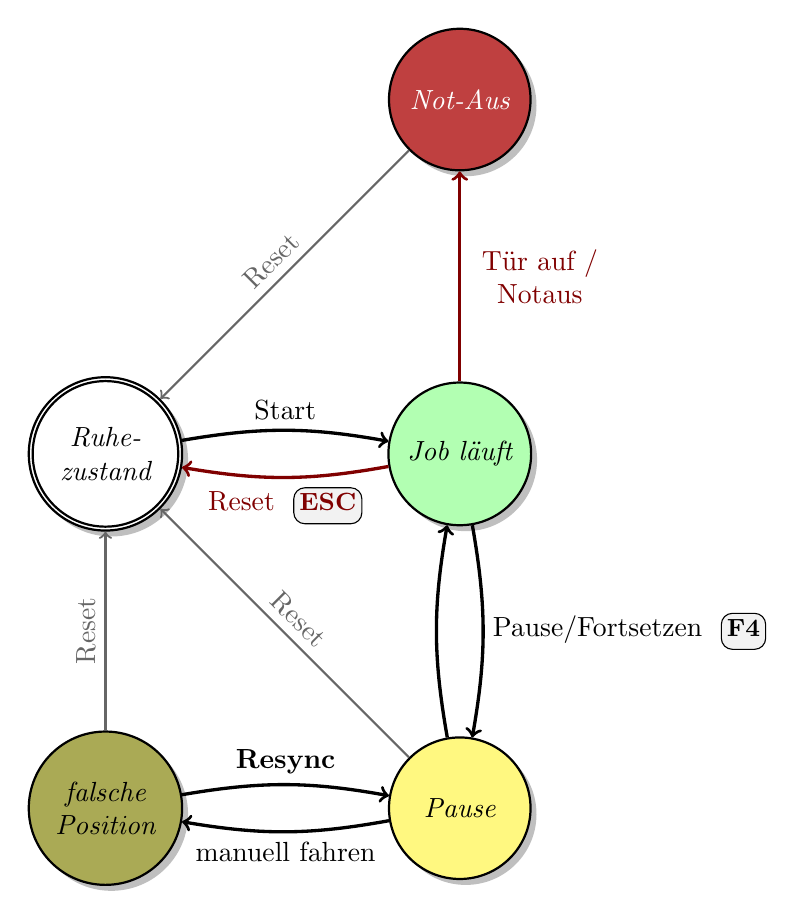
\begin{tikzpicture}[node distance=4.5cm,auto]
\colorlet{dunkelrot}{red!50!black}
\tikzstyle{zustand}=[shape=circle,draw,text width=1.5cm,text centered,thick,drop shadow,font=\it]; 
\tikzstyle{pf}=[->,very thick,every node/.style={anchor=south,text centered}]
\tikzstyle{pfHinRueck}=[pf,<->]

\node[zustand,fill=white] (ruhe) {Ruhe\-zustand};
\node[circle,text width=1.6cm,draw,thick] at (ruhe) {}; % innere zweite Umrandung - sieht so hübscher aus als mit der Option "double"
%\node[right of=ruhe] (platzhalter1) {}; % Lücke zwischen Ruhezustand und Job läuft
\node[zustand,right of=ruhe,fill=green!30!white] (aktiv) {Job läuft};

\node[zustand,above of=aktiv,fill=red!50!gray,text=white] (notaus) {Not-Aus};

\node[zustand,below of=aktiv,fill=yellow!50!white] (pause) {Pause};
\colorlet{schmutziggelb}{rgb:yellow,1;white,1;black,1}

\node[zustand,left of=pause,fill=schmutziggelb] (pauseVerschoben) {falsche Position};

\draw[pf,bend left=10] (ruhe) to node {Start}  (aktiv);
\draw[pf,bend left=10,dunkelrot] (aktiv) to node[anchor=north] {Reset \knopf{ESC}} (ruhe);

\draw[pf,bend left=10] (aktiv) to node[right] {Pause/Fortsetzen \knopf{F4}} (pause);
\draw[pf,bend left=10] (pause) to  (aktiv);
\draw[pf,bend left=10] (pause) to node[anchor=north] {manuell fahren} (pauseVerschoben) ;
\draw[pf,bend left=10] (pauseVerschoben) to node {\textbf{Resync}} (pause);

\draw[pf,dunkelrot] (aktiv) to node[right,text width=5em] {Tür auf /\\Notaus} (notaus);

\tikzstyle{unwichtig}=[color=black!60!white,thick]
\draw[pf,unwichtig] (notaus) to  node[sloped] {Reset} (ruhe);

\draw[pf,unwichtig,sloped] (pause) to node[sloped] {Reset} (ruhe);
\draw[pf,unwichtig,sloped] (pauseVerschoben) to node {Reset} (ruhe);
\end{tikzpicture}
\end{center}

Damit nach einer Unterbrechung wieder vom gleichen Zustand aus fortgesetzt wird, auch wenn man den Fräser zwischendurch manuell verfahren hat, erscheint nach \knopf{Start} der Resync-Dialog.

Jeder der Knöpfe steht für eine Variable. Grün heißt, dass der Zustand passend zum Fortsetzen ist. Draufklicken schaltet den Zustand um bzw. fährt zum passenden Fortsetzungspunkt.

\textbf{Bei Verwirrung geht stattdessen auch:} \knopf{Reset} setzt das Programm auf den Anfang zurück, jetzt kann man es nochmal vom Start aus laufen lassen. Es fräst dann anfangs in der Luft, das stört aber nicht weiter.

Die sinnvolle Reihenfolge beim Bedienen ist:
\begin{enumerate}
 \item Nach \knopf{Start} ist der Resync-Dialog links erschienen.
		\item Geschwindigkeit F (Textfeld), mit der zur Z-Höhe zurückgefahren wird, sollte auf 100 stehen (Kriechgang), sonst Crashgefahr.\\ Diese Geschwindigkeit gilt nicht für X/Y!
		\item Spindel an: \knopf{S}
		\item Kühlung an: \knopf{M8} kann manchmal auch rot sein, Hauptsache sie ist an
		\item Die Position kann auch wie gewohnt per Tastatur verfahren werden.
		\item Wenn die X/Y-Position nicht stimmt (Knopf mit roter Schrift), am besten erstmal den Fräser mit BildHoch aus dem Werkstück rausfahren, damit man nicht aus Versehen quer durchs Werkstück fährt.
			(Vorsicht bei sehr speziellen Fräserformen wie Gewindefräser, Kugelfräser o.\,ä.: Dabei kann es sein, dass man nicht einfach geradeaus hochfahren darf.)
		\item Position anfahren: \knopf{X}, \knopf{Y} (Abbrechen mit Esc)
		\item Danach Position \knopf{Z} anfahren (Abbrechen mit Esc)
		\item Erst wenn alles auf grün: \knopf{Start}
\end{enumerate}

\subsection{Auftragsende, Bezahlung}
\begin{enumerate}
 \item \textbf{Beachte:} Die angezeigte Zeit stimmt zur Zeit nicht, wenn man zwischendrin pausiert. \\\todo{Das ist ein Bug, der bereits gemeldet, aber noch nicht behoben wurde.}\\ Bitte orientierte dich an der vorausgesagten Zeit, die nach dem Neuladen der Datei angezeigt wird.
 \item Eingeben und Bezahlen im Kassenterminal, Details siehe Fräserpreisliste.
 \item Aufräumen wie unter \ref{ordnung} beschrieben.
\end{enumerate}


\section{Troubleshooting}

\subsection{Schrittverlust}
Bei zu großer Kraft kann die Fräse Schritte verlieren, d.h. es gibt jetzt einen Versatz zwischen der echten Position und der, die die Steuerung haben will. Das kann die Steuerung nicht merken! Abhilfe ist im Zweifelsfall eine erneute Referenzfahrt, das kann nie schaden und zeigt an, ob es Schrittverlust gab. Wenn nur 1 Schritt Verlust angezeigt wird, kann man das als Messfehler ignorieren.

\subsection{Fräserbruch}
\begin{itemize}
 \item Schrittverlust ist zu befürchten $\rightarrow$ Referenzfahrt!
 \item Vorderes abgebrochenes Teil des Fräsers anschauen: optisch in Ordnung? verklebt (Alu/Kunststoff)? noch scharf?
 \item Restliche Hartmetallteile aus dem Werkstück entfernen, sonst wird der nächste Fräser bei Berührung gleich wieder zerstört.
 \item Aufbauschneide? wenn ja: mehr KSS verwenden!
 \item Aufspannung starr genug? Blech wird gerne hochgezogen, sodass die Zustellung zu groß wird
 \item Ausreichend Schmierung?
 \item Zustellung verringern bei gleichem Vorschub, oder Vorschub verringern. Hat beides seine Vor- und Nachteile.
 \item Stege zu klein $\rightarrow$ Werkstück verschiebt sich und klemmt in den Fräser $\rightarrow$ Stege größer machen oder umspannen
 \end{itemize}


\subsection{MCA/TCA Collision}
Werkzeug vermessen? Nullpunkt korrekt?

Die angezeigte Koordinate ist nicht immer die Ursache der Fehlermeldung.

MCA: Fräsung zu tief ($<2$\,mm vom Tisch) oder außerhalb des Verfahrbereichs der Maschine. Beachte: Ein Fräser, der kürzer als 30\,mm herausragt, kommt nicht bis an den Tisch runter, weil die Z-Achse zu kurz ist!

TCA: Kollision mit \enquote{verbotenem Bereich} rund um den Längenmesstaster, also zu nahe dran. Mehr Abstand halten.

\section{Grundlagen}
\todo{ein kurzer Abschnitt über die nötigen Daten, und Begriffe erklären. Planfräsen, Nutfräsen, Stege,...}


\ccLicense{fraese-einweisung}{Einweisung Fräse}

\end{document}
